%%
%% This is file `sample-sigconf-authordraft.tex',
%% generated with the docstrip utility.
%%
%% The original source files were:
%%
%% samples.dtx  (with options: `all,proceedings,bibtex,authordraft')
%%
%% IMPORTANT NOTICE:
%%
%% For the copyright see the source file.
%%
%% Any modified versions of this file must be renamed
%% with new filenames distinct from sample-sigconf-authordraft.tex.
%%
%% For distribution of the original source see the terms
%% for copying and modification in the file samples.dtx.
%%
%% This generated file may be distributed as long as the
%% original source files, as listed above, are part of the
%% same distribution. (The sources need not necessarily be
%% in the same archive or directory.)
%%
%%
%% Commands for TeXCount
%TC:macro \cite [option:text,text]
%TC:macro \citep [option:text,text]
%TC:macro \citet [option:text,text]
%TC:envir table 0 1
%TC:envir table* 0 1
%TC:envir tabular [ignore] word
%TC:envir displaymath 0 word
%TC:envir math 0 word
%TC:envir comment 0 0
%%
%%
%% The first command in your LaTeX source must be the \documentclass
%% command.
%%
%% For submission and review of your manuscript please change the
%% command to \documentclass[manuscript, screen, review]{acmart}.
%%
%% When submitting camera ready or to TAPS, please change the command
%% to \documentclass[sigconf]{acmart} or whichever template is required
%% for your publication.
%%
%%
\documentclass[sigconf,authordraft]{acmart}
\usepackage{natbib}
\usepackage{url}
\usepackage{hyperref}
\usepackage{framed}
\usepackage{tcolorbox}
\usepackage{graphicx}
\usepackage{float}
\usepackage{enumitem}

%% Rights management information.  This information is sent to you
%% when you complete the rights form.  These commands have SAMPLE
%% values in them; it is your responsibility as an author to replace
%% the commands and values with those provided to you when you
%% complete the rights form.
\setcopyright{acmlicensed}
\copyrightyear{2024}
\acmYear{2024}
\acmDOI{XXXXXXX.XXXXXXX}

%% These commands are for a PROCEEDINGS abstract or paper.
\acmConference[Conference acronym 'XX']{Make sure to enter the correct conference title from your rights confirmation email}{June 03--05, 2018}{Woodstock, NY}
%%
%%  Uncomment \acmBooktitle if the title of the proceedings is different
%%  from ``Proceedings of ...''!
%%
%%\acmBooktitle{Woodstock '18: ACM Symposium on Neural Gaze Detection,
%%  June 03--05, 2018, Woodstock, NY}
\acmISBN{978-1-4503-XXXX-X/18/06}


%%
%% Submission ID.
%% Use this when submitting an article to a sponsored event. You'll
%% receive a unique submission ID from the organizers
%% of the event, and this ID should be used as the parameter to this command.
%%\acmSubmissionID{123-A56-BU3}

%%
%% For managing citations, it is recommended to use bibliography
%% files in BibTeX format.
%%
%% You can then either use BibTeX with the ACM-Reference-Format style,
%% or BibLaTeX with the acmnumeric or acmauthoryear sytles, that include
%% support for advanced citation of software artefact from the
%% biblatex-software package, also separately available on CTAN.
%%
%% Look at the sample-*-biblatex.tex files for templates showcasing
%% the biblatex styles.
%%

%%
%% The majority of ACM publications use numbered citations and
%% references.  The command \citestyle{authoryear} switches to the
%% "author year" style.
%%
%% If you are preparing content for an event
%% sponsored by ACM SIGGRAPH, you must use the "author year" style of
%% citations and references.
%% Uncommenting
%% the next command will enable that style.
%%\citestyle{acmauthoryear}


%%
%%
%% The "title" command has an optional parameter,
%% allowing the author to define a "short title" to be used in page headers.
\title{Roamify: Evaluating a Google Chrome Extension for Enhancing User Experience in Itinerary Planning}

%%
%% The "author" command and its associated commands are used to define
%% the authors and their affiliations.
%% Of note is the shared affiliation of the first two authors, and the
%% "authornote" and "authornotemark" commands
%% used to denote shared contribution to the research.
\author{Vikranth Udandarao}
\affiliation{%
  \institution{IIIT Delhi}
  \department{Computer Science Engineering Dept}
  \city{New Delhi}
  \country{India}}
\email{vikranth22570@iiitd.ac.in}

\author{Noel Abraham Tiju}
\affiliation{%
  \institution{IIIT Delhi}
  \department{Computer Science Engineering Dept}
  \city{New Delhi}
  \country{India}}
\email{noel22338@iiitd.ac.in}

\author{Muthuraj Vairamuthu}
\affiliation{%
  \institution{IIIT Delhi}
  \department{Computer Science Engineering Dept}
  \city{New Delhi}
  \country{India}}
\email{muthuraj22307@iiitd.ac.in}

\author{Harsh Mistry}
\affiliation{%
  \institution{IIIT Delhi}
  \department{Computer Science Engineering Dept}
  \city{New Delhi}
  \country{India}}
\email{harsh22200@iiitd.ac.in}


%%
%% By default, the full list of authors will be used in the page
%% headers. Often, this list is too long, and will overlap
%% other information printed in the page headers. This command allows
%% the author to define a more concise list
%% of authors' names for this purpose.
\renewcommand{\shortauthors}{Trovato et al.}

\begin{document}

%%
%% The abstract is a short summary of the work to be presented in the
%% article.
\begin{abstract}
This research delves into Roamify, an AI-powered travel assistance that makes travel preparations easy. It embarks on the usage of Large Language Models like Llama and T5 to generate personalised itineraries in accordance with user preferences. Results from user surveys highlight the preference for AI-powered mediums over existing methods to help in travel planning across all user age groups. These results firmly ideate the potential of Roamify. The following study highlights the three primary design considerations for travel assistance: \textbf{D1)} incorporating a web scrapping method to gather up-to-date news articles about various destinations and include them in our itineraries, \textbf{D2)} collecting various attractions and reviews from various blog sources, which significantly improves our itinerary suggestions, and \textbf{D3)} utilizing user preferences to create customized travel experiences along with a recommendation system which changes the itinerary according to the user needs. Our research indicates that Roamify has the immense potential to transform how users plan their trips once and forever.
\end{abstract}

\ccsdesc[500]{Human-centered computing~Ubiquitous and mobile computing systems and tools}
\ccsdesc[500]{Applied computing~Cartography}

  %%
  %% Keywords. The author(s) should pick words that accurately describe
  %% the work being presented. Separate the keywords with commas.
  \keywords{large language models, AI assistants, travel planning assistants, generative AI}
  %%
  %% This command processes the author and affiliation and title
  %% information and builds the first part of the formatted document.
  \maketitle

\section{Introduction}
    Traveling is truly a delightful experience for the human soul. Traditional planning methods
    required much information collection and were often restricted to people only in specific
    resource brackets. The general ways of planning for a trip or holiday consist of hours and hours of endless web surfing, reaching out to travel agencies and buying one of their travel packages. While these methods produced results, they weren’t quick or effective enough. All these planning methods have been proven to be tiring and cumbersome. At this dawn of rapid
    technological advancement, we can utilise technological mediums to aid us in our travel journey
    
    With the advancements in Large Language Models and Artificial intelligence, bygone are the
    days when we need to surf the internet continuously to ideate our dream journey.LLM’s have
    proven their mettle effortlessly trying to understand and replicate human interests through text and other visual representations. Over the years, they have shown varied success in different fields, including their ability to provide customised travel-related information. Consequently, claims regarding privacy concerns of LLMs have been arising, which calls the need for more generalization-focused solutions which aim for LLMs to operate effectively without disclosing private information. This context perfectly puts forth the need for Roamify and its travel-related services.
    
    Roamify utilizes LLMs to effectively categorise and provide perfectly personalized itinerary
    generation plans in a single click without the need for users to spend their valuable time
    gathering information. Furthermore, It also ensures that these services are compatible with
    different age groups, ensuring the product is universally accessible, thereby adhering to the
    Accessibility standards of HCI. Moreover,it maintains and ensures user privacy throughout their journey while utilising the platform which crafts their dream journey seamlessly.
    
    Moving towards the HCI aspect of Roamify, exhaustive user surveys and interviews stated the
    fact that majority of the age groups were affirmative towards using technological aids like
    Roamify to help in their travel planning. Millennials and Generation Z presented positive
    feedback and were excited to utilise platforms like Roamify, which would aid in their travel
    journey. Surprisingly, Generation X, although accustomed to the traditional methods of planning, were willing to look forward to what this new era of AI has to offer them in terms of travel planning. Their responses firmly underlined the great deal of potential Roamify has to offer.
    
    To further understand the effectiveness of our research work, we have outlined the following
    practical questions to help guide our research:
    
    \begin{itemize}
        \item \textbf{RQ1 - User Preferences and Personalization:} Would users like to have personalizations in their travel itineraries pertaining to their interests, history, adventures, calm sceneries, etc.?
        \item \textbf{RQ2 - Generated Responses:} Are the generated itinerary responses effective and can help their travel journey?
        \item \textbf{RQ3 - Current practices:} How do the users currently plan their travels and how do they feel about Roamify creating their travel plans employing AI mediums?
    \end{itemize}
    
    Through an aptly posed set of research questions, this paper attempts to illustrate the
    methodology behind the development of the Roamify application and then find scope within the
    tourism industry. Besides, through such in-depth exploration, we wish to present a complete
    understanding as to how mechanisms similar to Roamify can influence and assist in travel
    planning and aid in capturing human needs and preferences so that user experience can be
    improved accordingly

\section{Related Work}
  Large language models have a vast potential to be used for travel purposes, aiding travelers with their planning purposes as they save time and effort. However, a significant issue with using LLMs for travel is needing more tourism knowledge. Efforts have been in place to fine-tune LLMs to increase their resources for tourism and travel purposes\cite{ref3}. A detailed survey by Shengyu Gu discusses how these models can be used to explore possibilities such as personalized travel experiences and dynamic itineraries\cite{ref4}. Personalized travel experiences can be achieved by understanding user preferences and sentiments by analyzing textual data from reviews, direct customer interactions, and others. LLMs also possess the ability to generate informative travel guides that keep user preferences in mind, as well as generate compelling descriptions of attractions and sites to visit.

  We wanted to achieve the task of personalized itineraries by finding features that try to capture the user's taste in the best possible manner. We found diverse features such as natural, amusement, historical, and cultural. Keeping these genres to a minimum was also important because users were required to input these details before the itinerary generation began.

\newpage
\section{System Design and Architecture}

\begin{figure}
    \centering
    \includegraphics[width=1\linewidth]{system-design-image.png}
    \caption{System architecture}
    \label{fig:system-design}
\end{figure}
  Roamify is a Large Language Model based application primarily designed to create travel itineraries for users by considering their preferences on different genres as well as collecting up-to-date data regarding popular travel attractions. As discussed in the previous section, existing LLMs face challenges in planning itineraries as they are trained on relevant data at the time, which may no reflect current traveling trends.

  Roamify consists of four primary stages as part of its architecture as described in Figure \ref{fig:system-design}: \textbf{1) Data Collection}, \textbf{2) NLP Processing}, \textbf{3) Summarization}, and \textbf{4) Itinerary Generation}.

\subsection{Data Collection}
    The primary objective of the Data Collection phase is to gather relevant information from travel blogs and related websites. We implemented two methods for determining the user destination.

    \begin{itemize}
        \item \textbf{User Input:} The user directly inputs the desired destination along with the number of days they plan to spend thus allowing for a simple and reliable form of user input.

        \item \textbf{Web Scraping from Open Tabs:} The extension also has
        the ability to identify the destination by analyzing open tabs on the user's browser. This includes popular travel planning sites like MakeMyTrip as well as various travel blog such as TravelTriangle. By scraping these open tabs, the system can infer the user’s intended destination without the need for user input allowing for a more seamless user experience.
    \end{itemize}

    Once the target destination is determined, the system proceeds to gather up-to-date information by scraping data from highly-rated travel blog sites. The scraping process is carefully designed to effectively filter advertisements and other miscellaneous information that may not be deemed relevant for our use.

    Expanding the scraping corpus comes with two limitations:
    \begin{itemize}
        \item Increased latency
        \item Accumulation of redundant information
    \end{itemize}

  \subsection{NLP Processing}
    The second stage in the pipeline involves cleaning and processing the data gathered from the Data collection phase. This stage focuses extracting only the relevant information about attractions from the scraped text.

    Given that different websites follow different structures, we identified a common pattern across all the sources: attractions are typically numbered in ascending order. Using the insight, we applied the following steps to successfully determine the name of the attraction along with a short description.

    \begin{itemize}
        \item \textbf{Tokenization and Stopword Removal:} First, we tokenize the text and remove stopwords, after which we extract the sentences.

        \item \textbf{Pattern Recognition:} We search for an increasing sequence starting from one. This signifies the start of the list of popular attractions.

        \item \textbf{Information Extraction:} The text located between consecutive numbers is extracted and considered as the description or body for that particular attraction.

        \item \textbf{Dictionary Creation:} Finally, we format the extracted information into a dictionary format, where the names of the attractions and their descriptions are stored as key-value pairs.
    \end{itemize}

    This ensures that accurate and organized information is captured on each attraction laying the basis for our travel itinerary.

  \subsection{Summarization}
    This stage of the pipeline deals with condensing the information from the dictionary passed as input from the previous stage. Each key-value pair consists of the attraction name pointing to its details. However, advertisements along with other junk text may still be present in these descriptions if they were not filtered out successfuly by the previous stages. Clearing this persistent junk requires a more advanced tool such as Google Flan T5 or Llama-8b-Instruct models. Before fine-tuning the model, the task of summarization was performed adequately; however, to reduce the overall latency of the process, we required only relevant details to be passed on to the last stage.

    To achieve this, we fine-tuned both models using a custom dataset we prepared, which consisted of two components:

    \begin{itemize}
      \item \textbf{Context:} The attraction details extracted from the dictionary.
      \item \textbf{Summary:} The concise and relevant summary of the attraction details.
    \end{itemize}

    The following example demonstrates the context obtained after scraping, the summary used in the fine-tuning datasets, and the outputs generated by T5 and LLaMA, respectively:

\begin{tcolorbox}[linewidth=1pt, innerleftmargin=15pt, innerrightmargin=15pt, top=0pt, bottom=0pt]
\textbf{Context:}

Cubbon Park, Sarangib for Pixabay. Situated over a sprawling 300 acres of land, the park was constructed by Richard Sankey. This massive green park, along with lawns, deserves a special mention. Offering statues of famous personalities, the park is one among the popular places to visit in Bangalore with friends. Location: Kasturba Road, Behind High Court of Karnataka, Ambedkar Veedhi, Sampangi Rama Nagara, Bangalore. Timings: Open on all days. Entry Fee: No entry fee. Suggested Read: Resorts Near Bangalore.
\end{tcolorbox}\vspace{-10pt}
\begin{tcolorbox}[linewidth=1pt, innerleftmargin=15pt, innerrightmargin=15pt, innertopmargin=0pt, innerbottommargin=0pt]
\textbf{Summary (Dataset):}

Cubbon Park, spanning 300 acres and constructed by Richard Sankey, is a massive green space in Bangalore featuring lawns and statues of famous personalities. Located on Kasturba Road, it is a popular spot for outings with friends. The park is open daily with no entry fee.
\end{tcolorbox}\vspace{-10pt}
\begin{tcolorbox}[linewidth=1pt, innerleftmargin=15pt, innerrightmargin=15pt, innertopmargin=0pt, innerbottommargin=0pt]
\textbf{T5 Output:}

Cubbon Park, a sprawling 300 acres of land, is a popular place to visit in Bangalore with friends. Offering statues of famous personalities, it is a popular place to visit with friends.
\end{tcolorbox}\vspace{-10pt}
\begin{tcolorbox}[linewidth=1pt, innerleftmargin=15pt, innerrightmargin=15pt, innertopmargin=0pt, innerbottommargin=0pt]
\textbf{LLaMA Output:}

The park was constructed by Richard Sankey. This massive green park, along with lawns, deserves a special mention. Offering statues of famous personalities, the park is one among the popular places to visit in Bangalore with friends. Location: Kasturba Road, Behind High Court of Karnataka.
\end{tcolorbox}

From the above descriptions, we can see that T5 is more effective at capturing the essential information; hence, it successfully condenses the description while clearing out any junk text. On the other hand, Llama was more successful at elaborating on the description. However, this came with a much higher processing time than T5. Since processing time is an essential factor for our application, we integrated the T5 transformer into the pipeline as our mode for summarization.

\subsection{Itinerary Generation}
The final stage of the pipeline involves using Llama-3 or ChatGPT-4 to plan the itinerary based on the summarized and concise attractions given to it by the T5 transformer. The model then plans an itinerary using the attractions based on the number of days inputted by the user.

\begin{tcolorbox}[linewidth=1pt, innerleftmargin=15pt, innerrightmargin=15pt, innertopmargin=15pt, innerbottommargin=15pt]
  \textbf{Prompt Design:} \\

  Generate a detailed itinerary for me for a \underline{\textit{days}} day trip to  \underline{\textit{destination}} and here are the suggested places I would like to cover:

  \begin{itemize}
      \item \textbf{1. Attraction Name:}
      \begin{itemize}
          \item \textit{Description:} Attractions Details
      \end{itemize}
      \item \textbf{2. Attraction Name:}
      \begin{itemize}
          \item \textit{Description:} Attractions Details
      \end{itemize}
      \vspace{2\baselineskip} % Adds two line spaces
      \item \textbf{N. Attraction Name:}
      \begin{itemize}
          \item \textit{Description:} Attractions Details
      \end{itemize}
  \end{itemize}
\end{tcolorbox}

\begin{figure*}[h!]
    \centering
    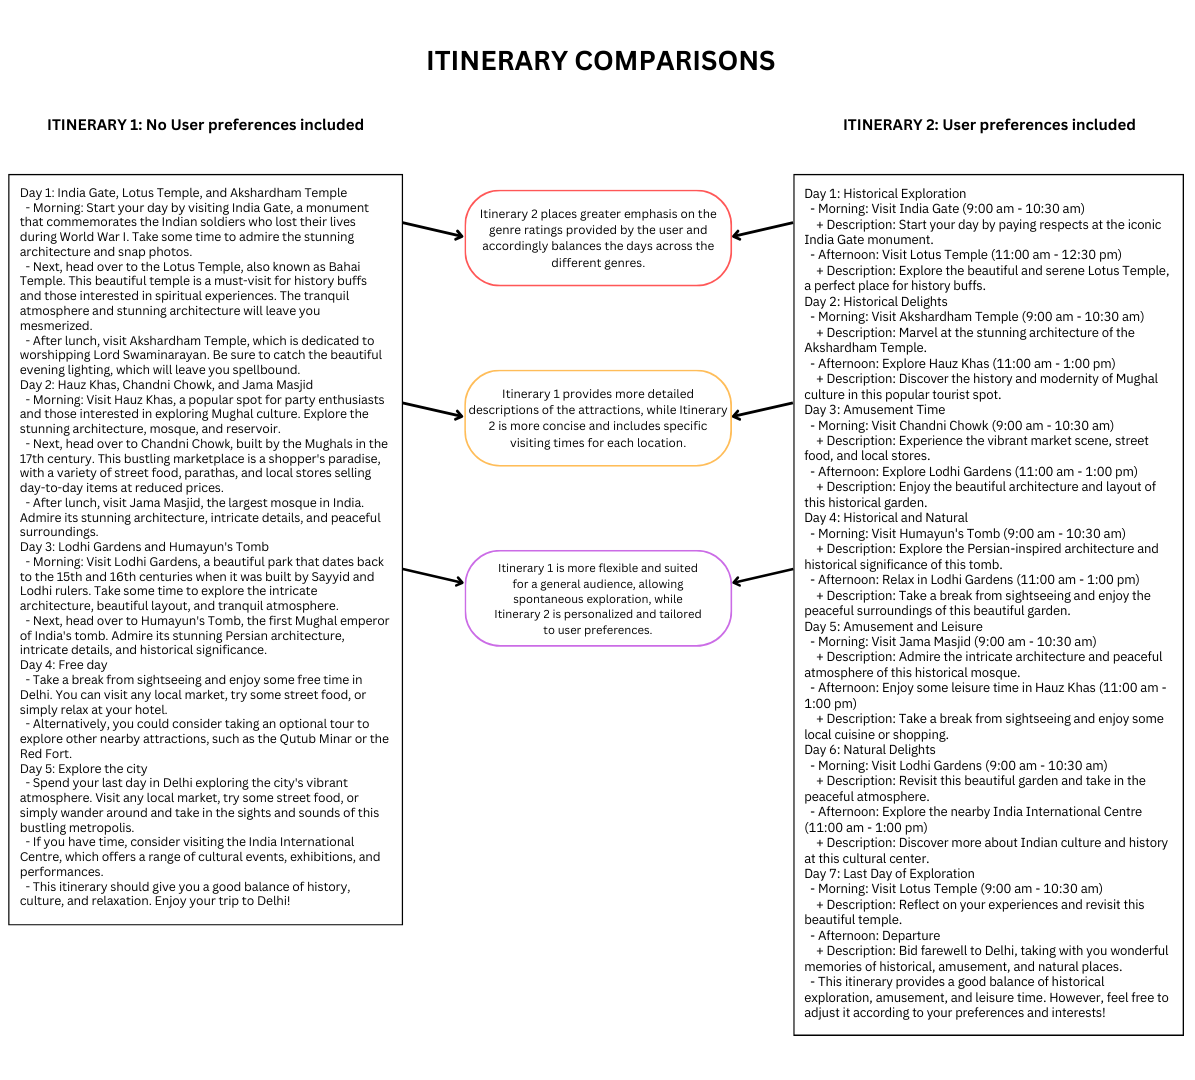
\includegraphics[width=0.8\textwidth]{Itinerary comparison.png}
    \caption{Comparison of Itineraries With and Without User Preferences Included}
    \label{fig:itinerary_comparison}
\end{figure*}

The above prompt is used to generate a general itinerary response using Ollama. A sample itinerary is produced in the Appendix.

However, these itineraries still needed to achieve the purpose of personalized recommendations based on users' preferences. On interviewing users, we identified some key features or distinct attraction genres that are important to them:

\begin{itemize}[noitemsep, topsep=5pt, parsep=0pt, partopsep=0pt]
    \item \textbf{Historical}
    \item \textbf{Amusement}
    \item \textbf{Natural}
    \item \textbf{Cultural}
\end{itemize}

For each genre, the user is shown a slider from 1 to 5 to rate it. These ratings are stored and added to the prompt so the itinerary can be planned accordingly. The updated prompt is shown below:

\subsection{Comparison of the Itineraries}

In Figure \ref{fig:itinerary_comparison}, a detailed comparison between two itineraries is presented: one that does not take user preferences into account (Itinerary 1) and another that does (Itinerary 2). There are three salient differences that can be observed between the two itineraries:

\begin{itemize}[noitemsep, topsep=5pt, parsep=0pt, partopsep=0pt]
\item \textbf{Genre Emphasis:} Itinerary 2 places greater emphasis on the genre ratings provided by the user and accordingly balances the days across the different genres.

\item \textbf{Detail Level:} Itinerary 1 provides more detailed descriptions of the attractions, while Itinerary 2 is more concise and includes specific visiting times for each location.

\item \textbf{Flexibility vs. Personalization:} Itinerary 1 is more flexible and suited for a general audience, allowing spontaneous exploration, while Itinerary 2 is personalized and tailored to user preferences.
\end{itemize}

Keeping these differences in mind, we sought to find which
itinerary is more beneficial for our use case. On asking interview participants, 75\% chose the itinerary that considered user preferences and admired the level of personalization that comes with it. Some participants were even told to go beyond the selected four features: historical, natural, amusement, and cultural, and add several more valuable features.
\newpage

\section{User Survey}

To understand user preferences and behaviors regarding travel, we conducted a survey and visualized the results in a series of pie charts. Below are the key findings:

\begin{itemize}
    \item \textbf{Types of Travel}: The largest portion of respondents (38\%) mentioned that they travel casually, indicating a preference for non-work-related trips. Entertainment-related travel also made up a significant portion (29.6\%), followed by work-related trips (11.3\%). Family trips were less common, constituting only 2.8\%, while minimal travel was motivated by meetups (8.5\%) or taking a break (1.4\%).

    \item \textbf{Travel Frequency}: The most common travel frequency reported by participants was once every six months (36.6\%), followed closely by once every three months (33.8\%). A smaller percentage of participants travel once a year (21.1\%), with even fewer traveling once a month (7\%) or twice a year (1.4\%).

    \item \textbf{Satisfaction with Travel Agencies}: Respondents were largely neutral about their experience with travel agencies, with 43.8\% selecting neutral. Those satisfied made up 29.7\%, while a small portion expressed being very satisfied (6.3\%). Dissatisfaction was also present, with 10.9\% feeling unsatisfied and 9.4\% being very unsatisfied.

    \item \textbf{Itinerary Decision}: Online travel websites were the most popular source for itinerary planning, with 46.5\% of participants using them. YouTube videos were also commonly used (31\%), while travel agents accounted for 14.1\%. Relatives and friends contributed to only 2.8\% of itinerary decisions, and a small fraction of participants preferred planning their itinerary themselves (4.2\%).

    \item \textbf{Help from Friends/Family for Itinerary}: A striking 88.7\% of respondents indicated that they seek help from friends or family for planning their itineraries, while only 11.3\% prefer doing it alone.

    \item \textbf{Demographic Distribution}: Young adults (ages 19-25) made up the majority of participants at 57.7\%. Adults between 26 and 64 years accounted for 29.6\%, while adolescents (ages 12-18) made up 9.9\%. Seniors (65 years and above) represented the smallest group at 2.8\%.

    \item \textbf{Customization Preferences}: A large majority of respondents (88.7\%) preferred to customize their own itineraries rather than rely on preselected ones (7\%), with a small group opting for a mix of both (4.2\%).

    \item \textbf{Custom Itinerary Build Time}: When asked how long it typically takes to build a custom itinerary, 32.4\% of respondents mentioned that it takes less than a day, while 28.2\% noted that it takes more than a week. A smaller proportion required 2-3 days (23.9\%) or exactly one day (15.5\%).
\end{itemize}

This detailed user survey analysis highlights the travel preferences and behaviors of the respondents, offering insights that can be used to tailor future travel planning services.

\begin{figure}
    \centering
    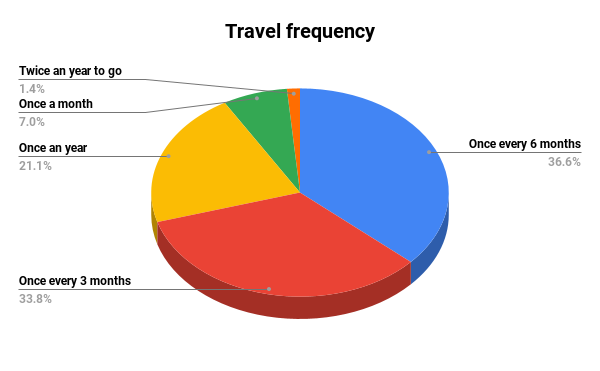
\includegraphics[width=0.5\linewidth]{Travel-frequency.png}
    \caption{Travel frequency}
    \label{fig:enter-label}
\end{figure}
\begin{figure}
    \centering
    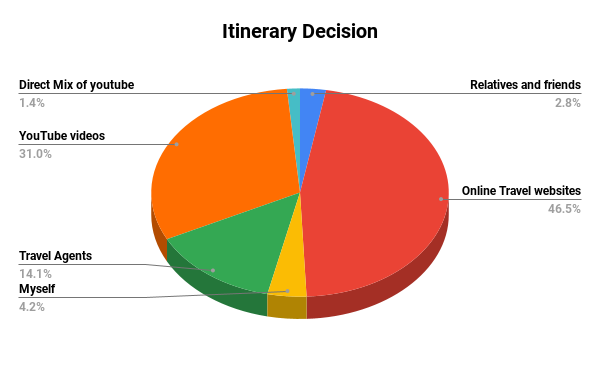
\includegraphics[width=0.5\linewidth]{Itinerary-Decision.png}
    \caption{Itinerary Decision}
    \label{fig:enter-label}
    \end{figure}
\begin{figure}
    \centering
    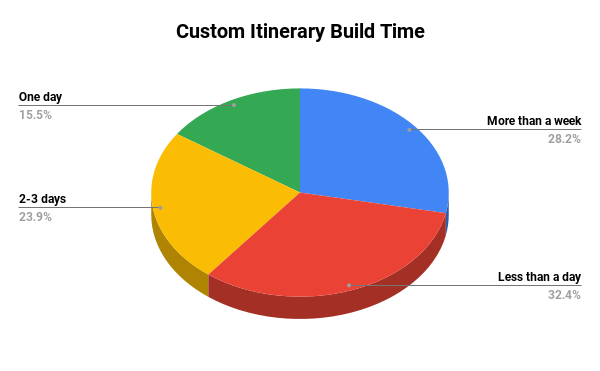
\includegraphics[width=0.5\linewidth]{Custom-Itinerary-Build-Time.png}
    \caption{Custom Itinerary Build Time}
    \label{fig:enter-label}
    \end{figure}
\begin{figure}
    \centering
    \includegraphics[width=0.5\linewidth]{Preference-for-an-AI-Travel-Planner.png}
    \caption{Preference for an AI Travel Planner}
    \label{fig:enter-label}
\end{figure}


\section{Interview Analysis and Testimonials}

    To further boost the credibility of our extension and find its certain shortcomings, we conducted around 100 interviews and collected testimonials from various travel influencers across the globe. Our aim was to learn the key impacts of their suggestions. Their ideology was unique and enhanced the sovereignty of our project, showing how we can further elevate it to an epitome scale.
    
    In our conversation with travel influencers and content creators, we came to a surprising realization: most of the travel influencers are bound by impromptu trips and sudden planning. They claimed this excited them the most and that they prefer impromptu trips over a week-long planned trip. This insight confirmed that our extension serves its purpose effectively.
    
    To further fuel our interests, we asked them about their regular ongoing trip processes and planning. We were amused by the nuances they consider when planning a trip. Their trip planning focused on finding exotic locations not frequently explored by other day-to-day travelers. They were more interested in the excitement of discovering new places and concerned with finding the logistics behind each trip.
    
    In light of this information, we carefully analyzed their needs and made sure our goals aligned with our customer interests. When we proposed the idea of an AI planning mechanism that could plan a trip in minutes, and asked for their feedback, the responses were overwhelmingly positive. Many of the travel influencers were excited about the new technologies and their role in everyday life. When we presented the idea that a planning attribute could be associated with an AI mechanism like Roamify, they were enthusiastic.
    
    They claimed that an AI travel mechanism would save time when making impromptu plans, allowing them to focus more on the nuances of the trip rather than spending time finding the correct resources and real-time information. They believed they could spend this energy learning more about the history behind the places and other essential aspects they'd like to explore. Additionally, many travel influencers felt that the current data available online is outdated and does not reflect the true travel experiences they seek. On the contrary, our AI platform, powered by Llama 3, ensures real-time updates and provides accurate, specific information instantly at the click of a button.
    
    When asked about the challenges they face while traveling, many influencers mentioned that they would like to find more accessible and affordable stays, along with itineraries, instantly. This is one of the critical pipelines in our upcoming work for Roamify, where we are working towards enhancing user accessibility and ensuring they get all their relevant details at their fingertips.
    
    When we presented our prototype, we received multiple appraisals and suggestions for improvement. The major pros included the GUI of the platform, which is very simple and easy to use, and the recommendation system that carefully crafts the needs and ideas to convert a trip into an enthralling journey. Suggestions for improvement included adding more logistical details and stay-related information to help create an enriching experience.
    
    From the exhaustive survey we conducted with travel influencers of various age groups, we were pleased to see that, despite the age gap, people were enthusiastic about using an AI mechanism to meet their travel needs and create a better experience with their loved ones. A detailed pie chart depicting this has been presented herewith.

\newpage
\begin{thebibliography}{99}

    \bibitem{ref3} Qikai Wei, Mingzhi Yang, Jinqiang Wang, Wenwei Mao, Jiabo Xu, Huansheng Ning. \textit{TourLLM: Enhancing LLMs with Tourism Knowledge}. 2024.

    \bibitem{ref4} Shengyu Gu. \textit{A Survey of Large Language Models in Tourism (Tourism LLMs)}. 2024.

    \bibitem{IEEEhowto:kopka}
        @article{article,
        author = {Filho, Angelo and Morabito, Reinaldo},
        year = {2023},
        month = {11},
        pages = {122437},
        title = {An effective approach for bi-objective multi-period touristic itinerary planning},
        volume = {240},
        journal = {Expert Systems with Applications},
        doi = {10.1016/j.eswa.2023.122437}
        }

    \bibitem{IEEEhowto:openai}
        OpenAI. (2023). "ChatGPT Release Notes." Retrieved from \url{https://help.openai.com/en/articles/6825453-chatgpt-release-notes}.

    \bibitem{IEEEhowto:econsultancy}
        Econsultancy. (2023). "Travel: How OTAs are adding generative AI to test the future of trip planning." Retrieved from \url{https://econsultancy.com/travel-ota-generative-ai/}.

    \bibitem{IEEEhowto:srdvtechnologies}
        SRDV Technologies. (2023). "Major Challenges Faced by Online Travel Agencies." Retrieved from \url{https://www.srdvtechnologies.com/blog/major-challenges-faced-by-online-travel-agencies}.

    \bibitem{ip2location}
        IP2Location, \emph{IP2Location IATA ICAO CSV}, \href{https://github.com/ip2location/ip2location-iata-icao/blob/master/iata-icao.csv}{https://github.com/ip2location/ip2location-iata-icao/blob/master/iata-icao.csv}.

    \bibitem{transformers}
        Hugging Face, \emph{Transformers Issue 27985 (with tracking parameters)}, \href{https://github.com/huggingface/transformers/issues/27985}{https://github.com/huggingface/transformers/issues/27985}.

    \bibitem{stackoverflow}
        Stack Overflow. Retrieved from \url{https://stackoverflow.com}.

    \bibitem{metawebsite}
        Meta. Retrieved from \url{https://about.meta.com}.

    \bibitem{youtube}
        YouTube, \emph{For training Llama Model using QLora and PEfT}, \href{https://www.youtube.com/watch?v=Vg3dS-NLUT4}{https://www.youtube.com/watch?v=Vg3dS-NLUT4}.

    \bibitem{llama}
        GitHub, \emph{Llama GitHub repository}, \href{https://github.com/facebookresearch/llama.git}{https://github.com/facebookresearch/llama.git}.

    \bibitem{spaCy}
        Explosion. (2023). "spaCy: Industrial-strength Natural Language Processing in Python." Retrieved from \url{https://spacy.io}.

    \bibitem{t5paper}
        Raffel, Colin, et al. "Exploring the limits of transfer learning with a unified text-to-text transformer." \emph{Journal of Machine Learning Research} 21.140 (2020): 1-67.

    \bibitem{bertpaper}
        Devlin, Jacob, et al. "BERT: Pre-training of Deep Bidirectional Transformers for Language Understanding." \emph{arXiv preprint arXiv:1810.04805} (2018).

    \bibitem{roberapaper}
        Liu, Yinhan, et al. "RoBERTa: A Robustly Optimized BERT Pretraining Approach." \emph{arXiv preprint arXiv:1907.11692} (2019).

    \bibitem{distilbertpaper}
        Sanh, Victor, et al. "DistilBERT, a distilled version of BERT: smaller, faster, cheaper and lighter." \emph{arXiv preprint arXiv:1910.01108} (2019).

    \bibitem{llamapaper}
        Touvron, Hugo, et al. "LLaMA: Open and Efficient Foundation Language Models." \emph{arXiv preprint arXiv:2302.13971} (2023).

    \bibitem{huggingface}
        Hugging Face. (2023). "Transformers: State-of-the-art Machine Learning for Pytorch, TensorFlow, and JAX." Retrieved from \url{https://github.com/huggingface/transformers}.

    \bibitem{nltk}
        Bird, Steven, Edward Loper, and Ewan Klein. "Natural language processing with Python: analyzing text with the natural language toolkit." \emph{"O'Reilly Media, Inc."} (2009).

    \bibitem{unsloth}
        Unsloth, \emph{Unsloth: An Efficient Library for Training Large Language Models}, \href{https://github.com/unsloth/unsloth}{https://github.com/unsloth/unsloth}.

    \bibitem{webscraping}
        Mitrevski, Marko. "Python Web Scraping: Hands-On Data Scraping and Crawling Using Pyspider, Splash, and Selenium." \emph{"Packt Publishing Ltd."} (2020).

    \bibitem{pythonselenium}
        SeleniumHQ. (2023). "Selenium WebDriver." Retrieved from \url{https://www.selenium.dev}.

    \bibitem{flant5}
        Heidloff, Niklas. (2023). "Fine-Tuning FLAN-T5." Retrieved from \url{https://heidloff.net/article/fine-tuning-flan-t5/}.

    \bibitem{flant5dc}
        DataCamp. (2023). "FLAN-T5 Tutorial." Retrieved from \url{https://www.datacamp.com/tutorial/flan-t5-tutorial}.

    \bibitem{flant5yt}
        YouTube. (2023). "FLAN-T5 Tutorial." Retrieved from \url{https://www.youtube.com/watch?v=PyRbP9d27sk}.

    \bibitem{llama3a}
        GitHub. (2023). "Unsloth: Efficient Library for Training Large Language Models." Retrieved from \url{https://github.com/unslothai/unsloth}.

    \bibitem{llama3b}
        Hugging Face Blog. (2023). "Fine-Tuning LLaMA-3 with Unsloth." Retrieved from \url{https://huggingface.co/blog/mlabonne/sft-llama3}.

    \bibitem{simpletransformers1}
        Towards Data Science. (2023). "Simple Transformers: Introducing the Easiest BERT, RoBERTa, XLNet, and XLM Library." Retrieved from \url{https://towardsdatascience.com/simple-transformers-introducing-the-easiest-bert-roberta}.
        % https://towardsdatascience.com/simple-transformers-introducing-the-easiest-bert-roberta-xlnet-and-xlm-library-58bf8c59b2a3

    \bibitem{simpletransformers2}
        YouTube. (2023). "Simple Transformers Tutorial." Retrieved from \url{https://www.youtube.com/watch?v=3XiJrn_8F9Q&t=1058s}.

\end{thebibliography}

\newpage

\appendix

\section{User Survey}
    To understand the travel planning behaviors and preferences of potential users for Roamify, we conducted a comprehensive survey. Below are the survey questions and the options provided for multiple-choice questions.
    \\

    \begin{enumerate}
        \item \textbf{What is your name?}

        \item \textbf{Which age group do you belong to?}
        \begin{itemize}
            \item Middle Childhood (6-11 years)
            \item Adolescents (12-18 years)
            \item Young Adults (19-25 years)
            \item Adults (26-64 years)
            \item Seniors (65 years+)
        \end{itemize}

        \item \textbf{How frequently do you travel?}
        \begin{itemize}
            \item Once a month
            \item Once every 3 months
            \item Once every 6 months
            \item Once a year
            \item Other
        \end{itemize}

        \item \textbf{What is the type of travel you usually undergo?}
        \begin{itemize}
            \item Work
            \item Entertainment
            \item Casual
            \item Meetup
            \item Other
        \end{itemize}

        \item \textbf{How do you decide your itinerary?}
        \begin{itemize}
            \item Travel Agents
            \item YouTube videos
            \item Online Travel websites
            \item Other
        \end{itemize}

        \item \textbf{How do you decide your itinerary?}
        \begin{itemize}
            \item Travel Agents
            \item YouTube videos
            \item Online Travel websites
            \item Other
        \end{itemize}

        \item \textbf{Do you like to travel based on your own customized itinerary or preselected recommended tourist packages?}
        \begin{itemize}
            \item Own Customized
            \item Preselected Recommended Tourist Packages
            \item Other
        \end{itemize}

        \item \textbf{If you have used a travel agency how much are you satisfied with their itinerary?}
        \begin{itemize}
            \item 1
            \item 2
            \item 3
            \item 4
            \item 5
        \end{itemize}

        \item \textbf{If you make custom itinerary how long do you take to build one?}
        \begin{itemize}
            \item Open-ended response
        \end{itemize}

        \item \textbf{Do you ask your friends and family for help who are currently living or have visited that place?}
        \begin{itemize}
            \item Yes
            \item No
        \end{itemize}
    \end{enumerate}

    \section{Interview Questions}
\\
    In addition to the survey, we conducted in-depth interviews with selected participants to gain deeper insights into their travel planning experiences. Below are the interview questions:
    \\

    \begin{enumerate}
        \item How frequently do you travel?
        \item Can you describe your typical process for planning a trip?
        \item What challenges do you face when planning a trip online?
        \item Have you ever used an offline travel agency? How was your experience compared to planning trips online?
        \item What features would you find most helpful in a travel planning tool?
        \item How important is the personalization of travel recommendations to you?
        \item Can you provide an example of a travel planning experience that was particularly stressful or frustrating?
        \item How do you think AI can improve the travel planning experience?
        \item What do you expect from a travel planning app or tool in terms of user experience?
        \item Have you ever used an AI-driven travel planning website where you can ask for personalized travel suggestions? If so, how was your experience?
    \end{enumerate}

% \begin{acks}
% To Robert, for the bagels and explaining CMYK and color spaces.
% \end{acks}
% %%
% %% The next two lines define the bibliography style to be used, and
% %% the bibliography file.
% \bibliographystyle{ACM-Reference-Format}
% \bibliography{sample-base}


% %%
% %% If your work has an appendix, this is the place to put it.
% \appendix

% \section{Research Methods}

% \subsection{Part One}

% Lorem ipsum dolor sit amet, consectetur adipiscing elit. Morbi
% malesuada, quam in pulvinar varius, metus nunc fermentum urna, id
% sollicitudin purus odio sit amet enim. Aliquam ullamcorper eu ipsum
% vel mollis. Curabitur quis dictum nisl. Phasellus vel semper risus, et
% lacinia dolor. Integer ultricies commodo sem nec semper.

% \subsection{Part Two}

% Etiam commodo feugiat nisl pulvinar pellentesque. Etiam auctor sodales
% ligula, non varius nibh pulvinar semper. Suspendisse nec lectus non
% ipsum convallis congue hendrerit vitae sapien. Donec at laoreet
% eros. Vivamus non purus placerat, scelerisque diam eu, cursus
% ante. Etiam aliquam tortor auctor efficitur mattis.

\end{document}
\endinput
%%
%% End of file `sample-sigconf-authordraft.tex'.
